\documentclass[a4paper,12pt]{article}
\usepackage[ukrainian,english]{babel}
\usepackage{ucs}
\usepackage[utf8]{inputenc}
\usepackage[T2A]{fontenc}
\usepackage{amsmath}
\usepackage[export]{adjustbox}
\usepackage{amsfonts}
\usepackage{graphicx}
\usepackage{changepage}
\usepackage{multirow}
\usepackage{subcaption}
\usepackage{wrapfig}
\usepackage{array, makecell}
\usepackage[document]{ragged2e}
\usepackage{parskip}
\usepackage[paper=portrait,pagesize]{typearea}
\usepackage{multicol}
\newcommand\tab[1][1cm]{\hspace*{#1}}
\newcommand\dd{\textbf{ d}}
\newcommand\const{\textbf{const}}
\addto\captionsenglish{\renewcommand{\figurename}{Рис.}}
\addto\captionsenglish{\renewcommand{\tablename}{Таблиця}}
\usepackage{titlesec}
\usepackage[left=20mm, top=20mm, right=20mm, bottom=20mm, nohead, nofoot]{geometry}
%\titleformat{\section}[block]{\Large\bfseries\filcenter}{}{1em}{}
\titleformat{\subsection}[hang]{\bfseries}{}{1em}{}
\titleformat{\subsubsection}[hang]{\bfseries}{}{2em}{}
\begin{document}
 \begin{justify}
 \thispagestyle{empty}\setlength{\parindent}{0pt}
  \topskip0pt
 \vspace*{\fill}
  \begin{center}
  \noindent\makebox[\linewidth]{\rule{\paperwidth}{0.4pt}}
   \LARGE{\bigbreak РОЗРАХУНКОВА РОБОТА З ЗАГАЛЬНОЇ ФІЗИКИ\\РОЗДІЛ "ЕЛЕКТРОДИНАМІКА"\\Варіант №2\bigbreak} 
   ФІ-12 Бекешева Анастасія 
   \noindent\makebox[\linewidth]{\rule{\paperwidth}{0.4pt}}
  \end{center}
 \vspace*{\fill}\newpage
 \section{Умови}
 \begin{itemize}
  \item $\varepsilon=1$
  \item $\rho(r)=\rho_0\left(\dfrac{R_2}{r}\right)$
  \item $\rho_0=50\cdot10^{-9}\dfrac{\textrm{Кл}}{\textrm{м}^3}$
  \item $R_1=0.05\textrm{м}$
  \item $R_2=0.1\textrm{м}$
  \item $\sigma=0$
 \end{itemize}
 \section{Рисунок}
 \begin{figure}[!h]
    \centering
    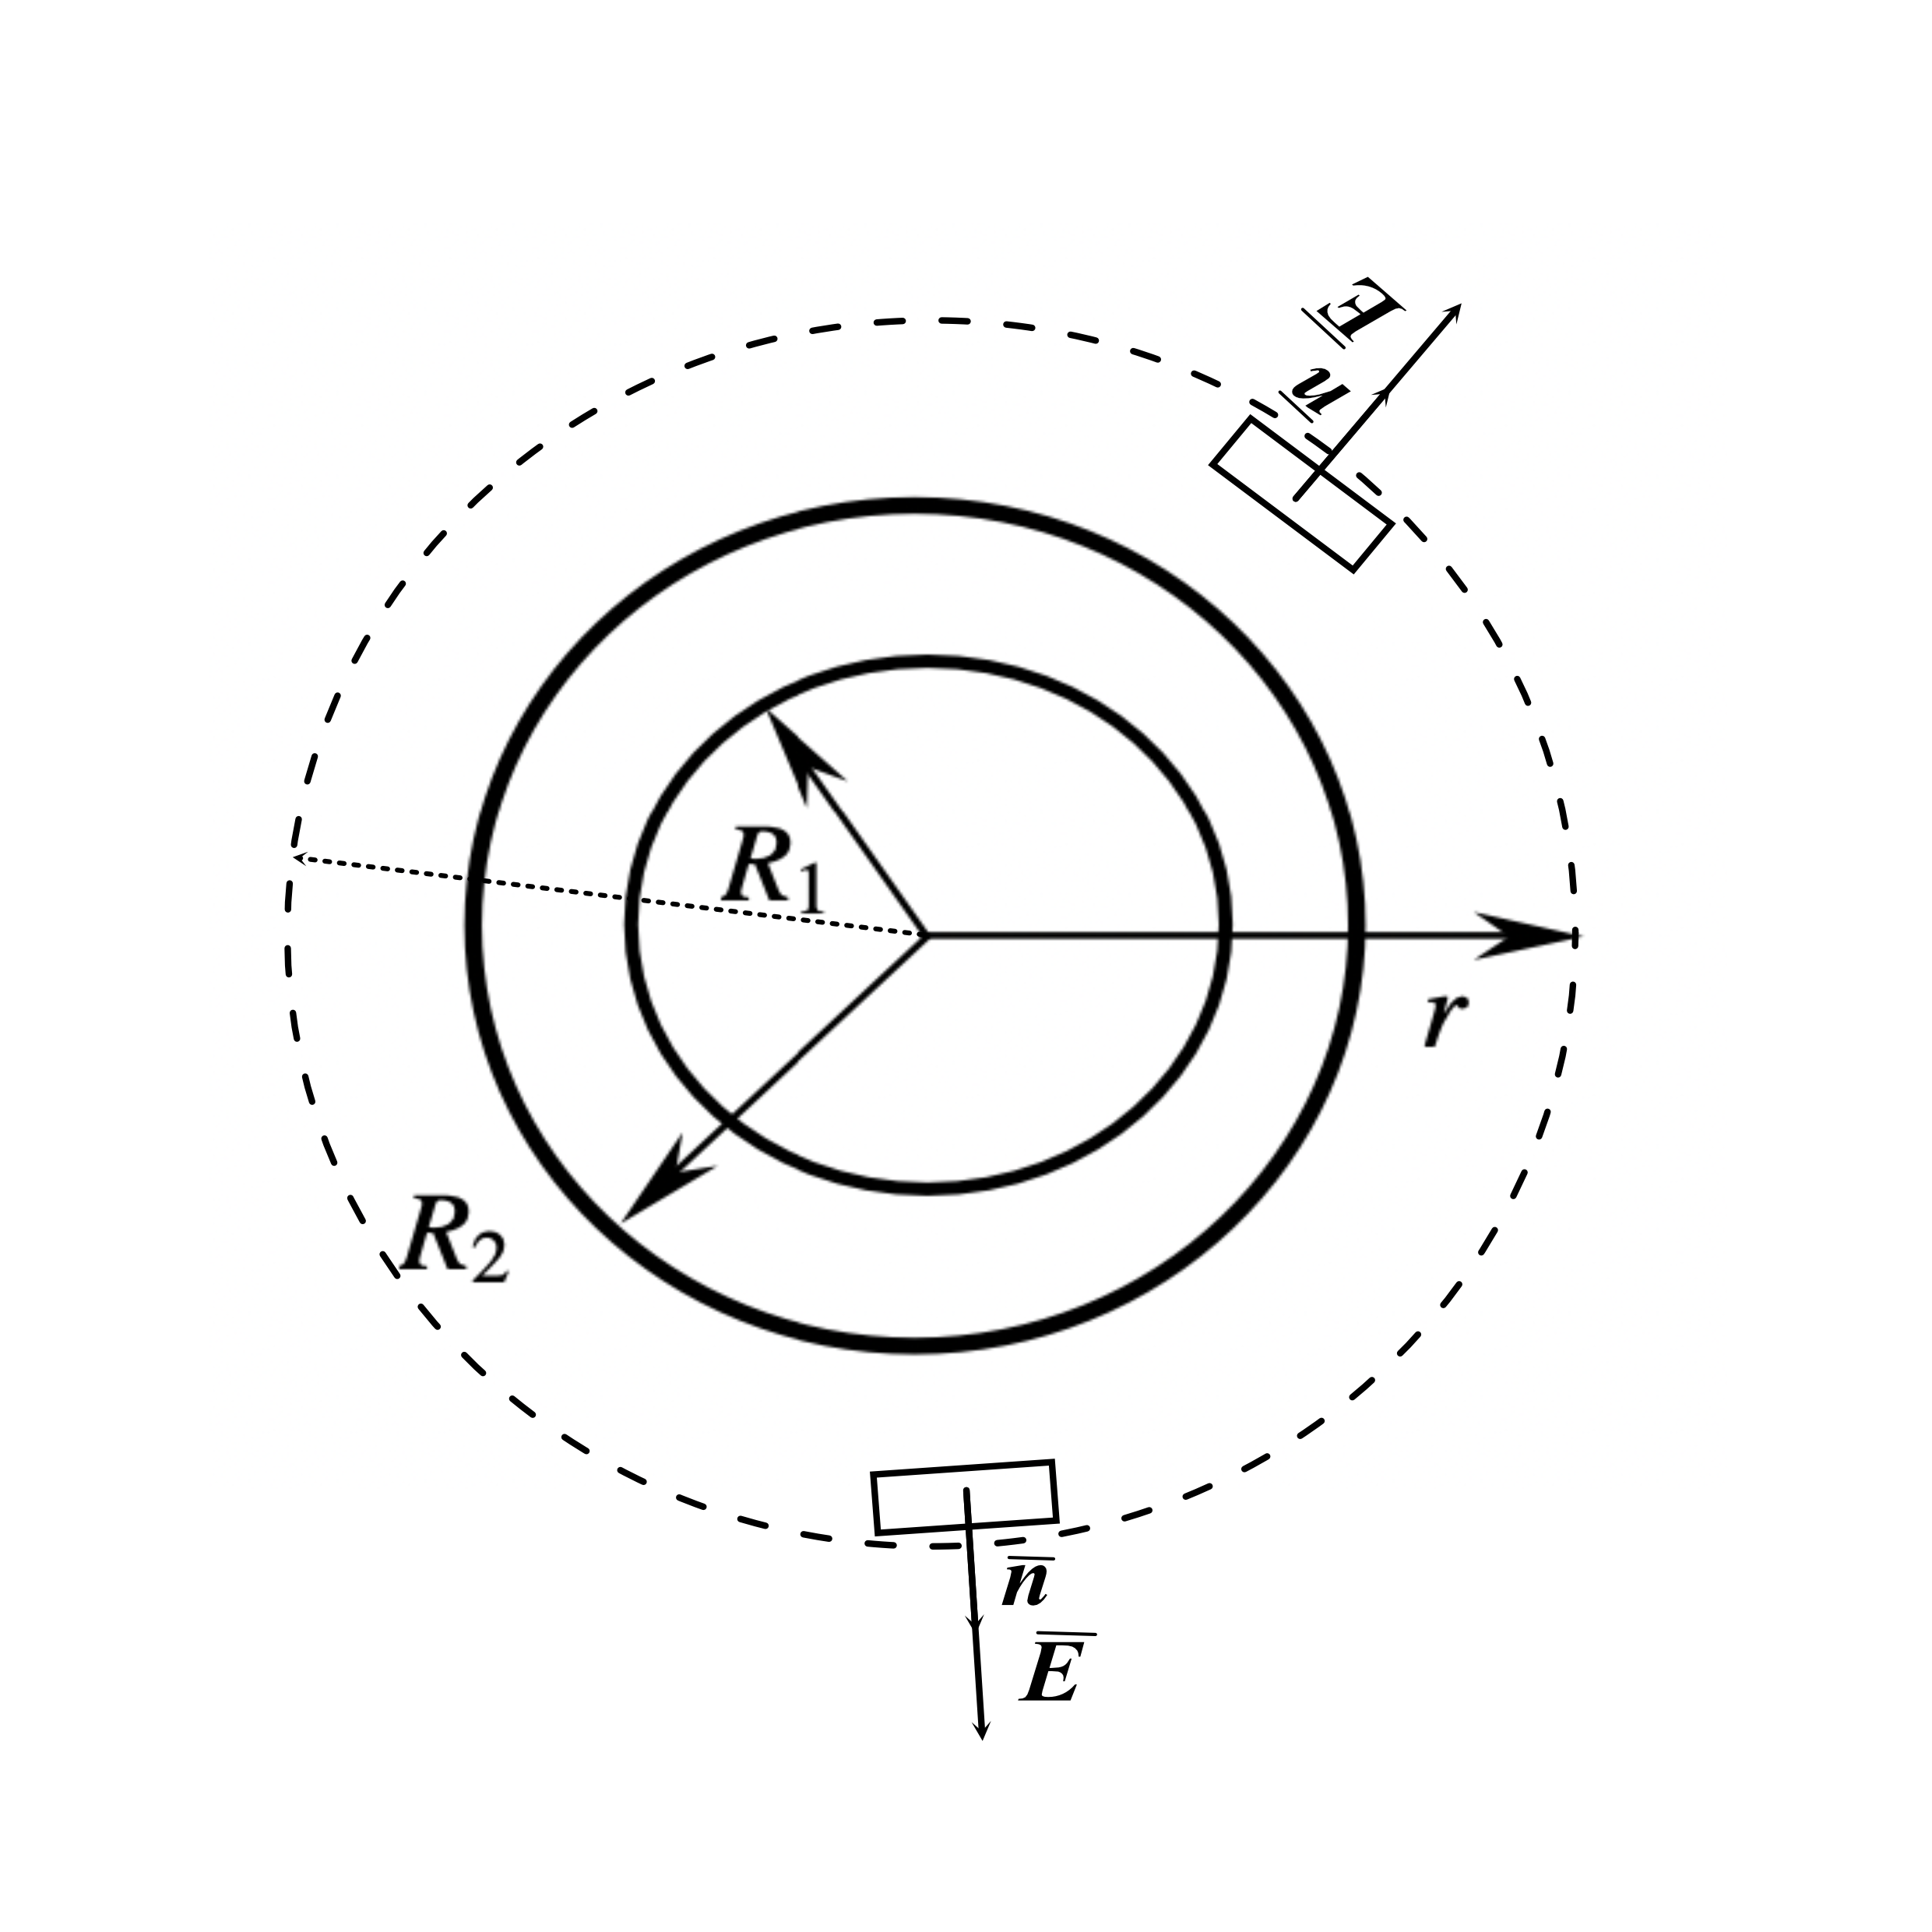
\includegraphics[width=10cm]{media/cw_graph1}
    \caption{Кульовий шар із зовнішнім та внутрішнім радіусами}
    \label{fig:1}
 \end{figure}
 \section{Вирази для $E_r(r)$}
 $\displaystyle\oint E\dd S=\dfrac{Q}{\varepsilon_0},\tab Q=\displaystyle\int\limits_{R_1}^{R_2}\rho\dd V+\sigma\cdot S$
 \subsection{$r<R_1$}
 Поле відсутнє. Зарядів у поверхні немає. $E=0$
 \begin{equation}
  E_1=0
 \end{equation}
 \subsection{$R_1\leq r\leq R_2$}
 $\rho=\dfrac{\dd Q_2}{\dd V},\tab \dd Q_2=\rho\cdot\dd V,\tab \dd V=S\dd r=4\bar{n}r^@\dd r,\tab Q_2=\displaystyle\int\rho\cdot S\dd r,\\Q_2=\displaystyle\int\limits_{R_1}^r\rho\cdot4\bar{n}r^2\dd r=\displaystyle\int\limits_{R_1}^r\rho_0\cdot4\bar{n}r^2\dfrac{R_2}{r}\dd r=\displaystyle\int\limits_{R_1}^r\rho_0\cdot4\bar{n}\cdot R_2\cdot r\dd r=\rho_0\cdot4\bar{n}\cdot R_2\displaystyle\int\limits_{R_1}^r r\dd r=\\=\rho_0\cdot4\bar{n}\cdot R_2\cdot\left.\dfrac{r^2}{2}\right|_{R_1}^r=2\rho_0\cdot\bar{n}\cdot R_2\\E=\dfrac{Q_2}{S\cdot\varepsilon_0}=\dfrac{2\rho_0\cdot\bar{n}\cdot R_2\cdot(r^2-R_1^2)}{4\bar{n}\cdot r^2\cdot\varepsilon_0}=\dfrac{\rho_0\cdot R_2\cdot(r^2-R^2_1)}{2r^2\cdot\varepsilon_0}$
 \begin{equation}
  E_2= \dfrac{\rho_0\cdot R_2\cdot(r^2-R^2_1)}{2r^2\cdot\varepsilon_0}
 \end{equation}
 \subsection{$r>R_2$}
 $Q_3=\displaystyle\int\rho\cdot D\dd r=\displaystyle\int\limits_{R_1}^{R_2}\rho_0\cdot4\bar{n}\cdot r^2\dfrac{R_2}{r}\dd r=\rho_0\cdot 4\bar{n}\cdot R_2\left.\dfrac{r^2}{2}\right|_{R_1}^{R_2}=2\rho_0\cdot\bar{n}\cdot R_2\cdot(R_1^2-R_2^2)\\E=\dfrac{Q_3}{S\cdot\varepsilon_0}=\dfrac{2\rho_0\cdot\bar{n}\cdot R_2\cdot(R_2^2-R_1^2)}{4\bar{n}\cdot r^2\cdot\varepsilon_0}=\dfrac{\rho_0\cdot R_2\cdot(R_2^2-R_1^2)}{2r^2\cdot\varepsilon_0}$
 \begin{equation}
  E_3=\dfrac{\rho_0\cdot R_2\cdot(R_2^2-R_1^2)}{2r^2\cdot\varepsilon_0}
 \end{equation}
 \section{Вирази для $\varphi(r)$}
 \subsection{$r<R_1$}
 $\varphi=\const=-\displaystyle\int E\dd r+C$
 \begin{equation}
  \varphi_1=\dfrac{\rho_0R_2\cdot(R_2-R_1)}{\varepsilon_0}
 \end{equation}
 \subsection{$R_1\leq r\leq R_2$}
 $\varphi=-\dfrac{\rho_0R_2}{2\varepsilon_0}\displaystyle\int\dfrac{(r^2-R_1^2)}{r^2}\dd r=-\dfrac{\rho_0R_2}{2\varepsilon_0}\left(r-\dfrac{R_1^2}{r}\right)+C$
 \begin{equation}
  \varphi_2=-\dfrac{\rho_0R_2}{2\varepsilon_0}\left(r-\dfrac{R_1^2}{r}\right)+C
 \end{equation}
 \subsection{$r>R_2$}
 $\varphi=-\displaystyle\int\dfrac{\rho_0R_2\cdot(R_2^2-R_1^2)}{2r^2\varepsilon_0}=\dfrac{\rho_0R_2\cdot(R_2^2-R_1^2)}{2r\varepsilon_0}+c\\\varphi(r\to\infty)=0\Rightarrow C=0$
 \begin{equation}
  \varphi_3=\dfrac{\rho_0R_2\cdot(R_2^2-R_1^2)}{2r\varepsilon_0}
 \end{equation}
 \section{Числові формули}
 $\varphi_2(R_2)=\varphi_3(R_2)\Rightarrow C=\dfrac{\rho_0R_2^2}{\varepsilon_0}$
 \begin{equation}
  \varphi_2=-\dfrac{\rho_0R_2}{2\varepsilon_0}\left(r-\dfrac{R_1^2}{r}\right)+\dfrac{\rho_0R_2^2}{\varepsilon_0}=\dfrac{-\rho_0R_2(r^2-R_1^2)+2\rho_0R_2^2}{2\varepsilon_0}=\dfrac{\rho_0R_2(2R_2-r^2+R_1^2)}{2\varepsilon_0}
 \end{equation}
 \section{Розрахунок}
 \begin{table}[htp]\centering
\begin{tabular}{|c|c|c|c|c|}
\hline
   & $r$  & $\rho$   & $E$    & $\varphi$ \\ \hline
0  & 0.0  & $\infty$ & 0.0    & 28.25     \\ \hline
1  & 0.01 & 10.0     & 0.0    & 28.25     \\ \hline
2  & 0.02 & 5.0      & 0.0    & 28.25     \\ \hline
3  & 0.03 & 3.33     & 0.0    & 28.25     \\ \hline
4  & 0.04 & 2.5      & 0.0    & 28.25     \\ \hline
5  & 0.05 & 2.0      & 0.0    & 28.25     \\ \hline
6  & 0.06 & 1.67     & 86.32  & 27.78     \\ \hline
7  & 0.07 & 1.43     & 138.36 & 26.63     \\ \hline
8  & 0.08 & 1.25     & 172.14 & 25.07     \\ \hline
9  & 0.09 & 1.11     & 195.3  & 23.23     \\ \hline
10 & 0.1  & 1.0      & 211.86 & 21.19     \\ \hline
11 & 0.11 & 0.91     & 175.09 & 19.26     \\ \hline
12 & 0.12 & 0.83     & 147.13 & 17.66     \\ \hline
13 & 0.13 & 0.77     & 125.36 & 16.3      \\ \hline
14 & 0.14 & 0.71     & 108.09 & 15.13     \\ \hline
15 & 0.15 & 0.67     & 94.16  & 14.12     \\ \hline
16 & 0.16 & 0.62     & 82.76  & 13.24     \\ \hline
17 & 0.17 & 0.59     & 73.31  & 12.46     \\ \hline
18 & 0.18 & 0.56     & 65.39  & 11.77     \\ \hline
19 & 0.19 & 0.53     & 58.69  & 11.15     \\ \hline
20 & 0.2  & 0.5      & 52.97  & 10.59     \\ \hline
\end{tabular}
\end{table}
\section{Графіки}
\begin{figure*}[!h]
  \centering
  \begin{subfigure}{0.6\linewidth}
   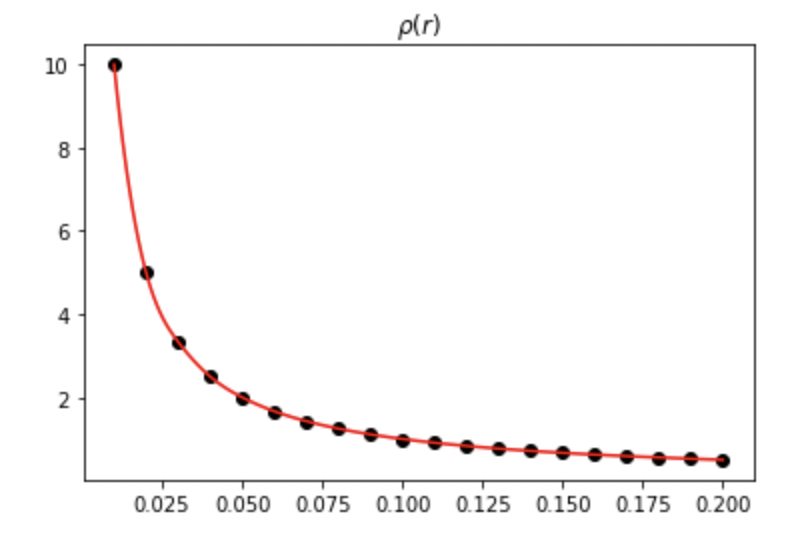
\includegraphics[height=65mm]{media/cw_graph2a}
      \caption{Залежність густини від $r$}
   \label{fig:6a}
     \end{subfigure}\hfill
          \begin{subfigure}{0.6\linewidth}
   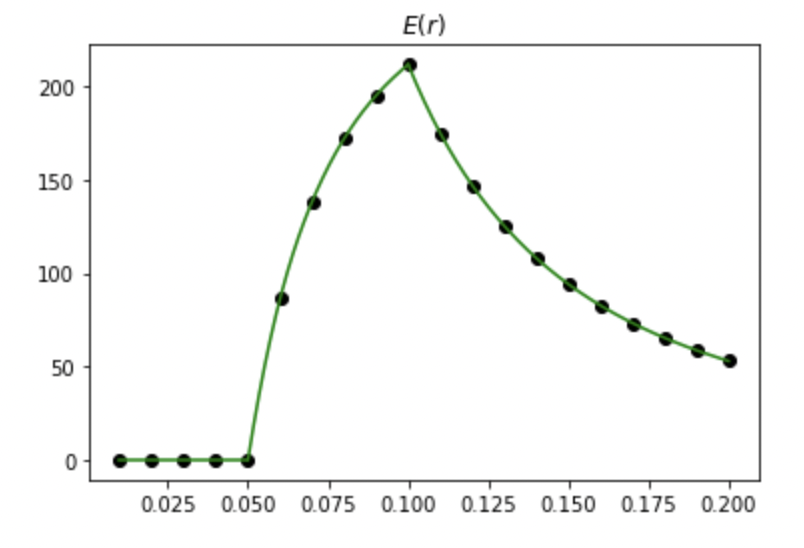
\includegraphics[height=65mm]{media/cw_graph2b}
      \caption{Залежність напруженості від $r$}
   \label{fig:6b}
     \end{subfigure}\hfill
     \begin{subfigure}{0.6\linewidth}
   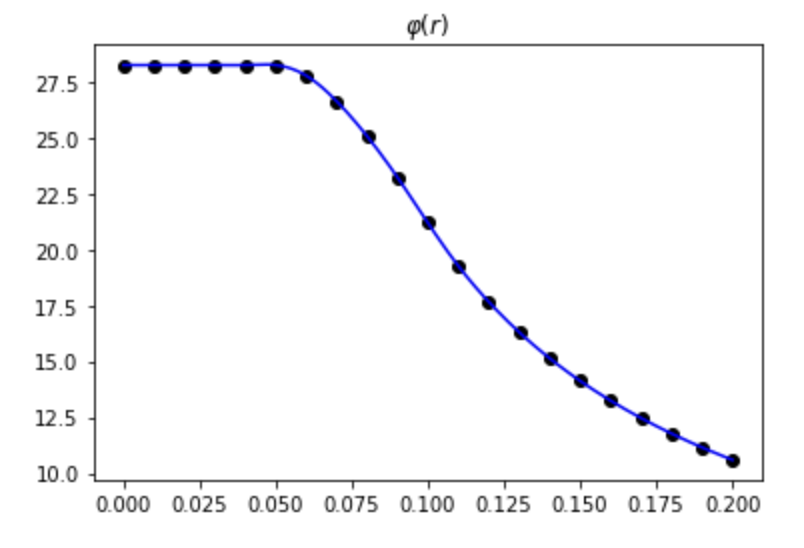
\includegraphics[height=65mm]{media/cw_graph2c}
      \caption{Залежність потенціалу від $r$}
   \label{fig:6c}
     \end{subfigure}\hfill
  \caption{Графіки залежностей}
  \label{fig:6}
 \end{figure*}$\\$
 
 
 
 
 
 
 
 
 
 
 
 
 
 
 
 
 
 
 
 
 
 
 
 
 
 
 
 
 
 
 
 \end{justify}
\end{document}